\documentclass{article}
\usepackage[utf8]{inputenc}
% \usepackage[russian]{babel}
\usepackage[a4paper, top=0.7in, left=0.5in, right=0.5in, bottom=0.6in, twocolumn]{geometry}
\usepackage{lastpage}
\usepackage{fancyhdr}
\usepackage{tikz}
\usepackage{pgfplots}
\usepackage{amssymb}
\usepackage{minted}
\usepackage{pdfpages}
\usepackage{booktabs}

\usetikzlibrary{shapes}

\setcounter{secnumdepth}{5}
\setcounter{tocdepth}{5}
\pgfkeys{/pgf/number format/.cd,1000 sep={\,}}

\pagestyle{fancy}
\fancyhf{}
\lhead{ITMO University 1: Insert your name (Budin, Korobkov, Naumov)}
\rhead{Page \thepage\ of \pageref{LastPage}}
\lfoot{Generated \today}

\renewcommand{\footrulewidth}{0.4pt}
\setlength{\columnseprule}{0.4pt}

\begin{document}
% \onecolumn
\tableofcontents

% \twocolumn
% \newpage

\section{Some usefull stuff}
\subsection{Fast I/O}
\inputminted[mathescape, breaklines, breakafter=(, tabsize=2, frame=lines, showtabs, tab=|\ , tabcolor=lightgray]{c++}{./basic/fast-io/io.cpp}
\subsection{Java template}
\inputminted[mathescape, breaklines, breakafter=(, tabsize=2, frame=lines, showtabs, tab=|\ , tabcolor=lightgray]{java}{./basic/java-template/Template.java}
\subsection{Pragmas}
\inputminted[mathescape, breaklines, breakafter=(, tabsize=2, frame=lines, showtabs, tab=|\ , tabcolor=lightgray]{c++}{./basic/pragmas/opt.cpp}
\section{Data structures}
\subsection{Hash table}
\inputminted[mathescape, breaklines, breakafter=(, tabsize=2, frame=lines, showtabs, tab=|\ , tabcolor=lightgray]{c++}{./data-structures/hash-table/hash-table.cpp}
\subsection{Ordered set and bitset}
\inputminted[mathescape, breaklines, breakafter=(, tabsize=2, frame=lines, showtabs, tab=|\ , tabcolor=lightgray]{c++}{./data-structures/std/std.cpp}
\section{Geometry}
\subsection{Common tangents of two circles}
\inputminted[mathescape, breaklines, breakafter=(, tabsize=2, frame=lines, showtabs, tab=|\ , tabcolor=lightgray]{c++}{./geometry/common-tangents/common-tangents.cpp}
\subsection{Convex hull 3D in $O(n ^ 2)$}
\inputminted[mathescape, breaklines, breakafter=(, tabsize=2, frame=lines, showtabs, tab=|\ , tabcolor=lightgray]{c++}{./geometry/convex-hull-3d/convex-hull-3d.cpp}
\subsection{Dynamic convex hull trick}
\inputminted[mathescape, breaklines, breakafter=(, tabsize=2, frame=lines, showtabs, tab=|\ , tabcolor=lightgray]{c++}{./geometry/convex-hull-trick/convex-hull-trick.cpp}
\subsection{Halfplanes intersection}
\inputminted[mathescape, breaklines, breakafter=(, tabsize=2, frame=lines, showtabs, tab=|\ , tabcolor=lightgray]{c++}{./geometry/halfplanes-intersection/halfplanes-intersection.cpp}
\subsection{Minimal covering disk}
\inputminted[mathescape, breaklines, breakafter=(, tabsize=2, frame=lines, showtabs, tab=|\ , tabcolor=lightgray]{c++}{./geometry/min-disk/min-disk.cpp}
\subsection{Polygon tangent}
\inputminted[mathescape, breaklines, breakafter=(, tabsize=2, frame=lines, showtabs, tab=|\ , tabcolor=lightgray]{c++}{./geometry/polygon-tangent/polygon-tangent.cpp}
\subsection{Draw svg pictures}
\inputminted[mathescape, breaklines, breakafter=(, tabsize=2, frame=lines, showtabs, tab=|\ , tabcolor=lightgray]{c++}{./geometry/svg-draw/svg-draw.cpp}
\section{Graphs}
\subsection{2-Chinese algorithm}
\inputminted[mathescape, breaklines, breakafter=(, tabsize=2, frame=lines, showtabs, tab=|\ , tabcolor=lightgray]{c++}{./graphs/2-chinese/2-chinese.cpp}
\subsection{Dominator tree}
\inputminted[mathescape, breaklines, breakafter=(, tabsize=2, frame=lines, showtabs, tab=|\ , tabcolor=lightgray]{c++}{./graphs/dominator-tree/dominator-tree.cpp}
\subsection{General matching}
\inputminted[mathescape, breaklines, breakafter=(, tabsize=2, frame=lines, showtabs, tab=|\ , tabcolor=lightgray]{c++}{./graphs/general-matching/general-matching.cpp}
\subsection{Gomory-Hu tree}
\inputminted[mathescape, breaklines, breakafter=(, tabsize=2, frame=lines, showtabs, tab=|\ , tabcolor=lightgray]{c++}{./graphs/gomory-hu/gomory-hu.cpp}
\subsection{Hungarian algorithm}
\inputminted[mathescape, breaklines, breakafter=(, tabsize=2, frame=lines, showtabs, tab=|\ , tabcolor=lightgray]{c++}{./graphs/hungarian-algorithm/hungarian-algorithm.cpp}
\subsection{Link-Cut Tree}
\inputminted[mathescape, breaklines, breakafter=(, tabsize=2, frame=lines, showtabs, tab=|\ , tabcolor=lightgray]{c++}{./graphs/link-cut-tree/link-cut-tree.cpp}
\subsection{Push-Relabel}
\inputminted[mathescape, breaklines, breakafter=(, tabsize=2, frame=lines, showtabs, tab=|\ , tabcolor=lightgray]{c++}{./graphs/push-relabel/push-relabel.cpp}
\subsection{Smith algorithm (Game on cyclic graph)}
\inputminted[mathescape, breaklines, breakafter=(, tabsize=2, frame=lines, showtabs, tab=|\ , tabcolor=lightgray]{c++}{./graphs/smith/smith.cpp}
\subsection{Stoer-Vagner algorithm (Global min-cut)}
\inputminted[mathescape, breaklines, breakafter=(, tabsize=2, frame=lines, showtabs, tab=|\ , tabcolor=lightgray]{c++}{./graphs/stoer-vagner/stoer-vagner.cpp}
\section{Matroids}
\subsection{Matroids intersection}
\inputminted[mathescape, breaklines, breakafter=(, tabsize=2, frame=lines, showtabs, tab=|\ , tabcolor=lightgray]{c++}{./matroids/matroids-intersection/matroids-intersection.cpp}
\section{Numeric}
\subsection{Berlekamp-Massey Algorithm}
\inputminted[mathescape, breaklines, breakafter=(, tabsize=2, frame=lines, showtabs, tab=|\ , tabcolor=lightgray]{c++}{./numeric/berlekamp/berlekamp.cpp}
\subsection{Burnside's lemma}
$$|X/G| = \frac{1}{|G|}\sum\limits_{g \in G}|St(g)|$$

$St(g)$ denote the set of elements in $X$ that are fixed by $g$, i.e. $St(g) = \{x \in X | gx = x\}$.
\subsection{Chinese remainder theorem}
\inputminted[mathescape, breaklines, breakafter=(, tabsize=2, frame=lines, showtabs, tab=|\ , tabcolor=lightgray]{c++}{./numeric/chinese-remainder-theorem/chinese-remainder-theorem.cpp}
\subsection{Convolutions}
\subsubsection{AND convolution}
\inputminted[mathescape, breaklines, breakafter=(, tabsize=2, frame=lines, showtabs, tab=|\ , tabcolor=lightgray]{c++}{./numeric/convolutions/and-conv/and-conv.cpp}
\subsubsection{OR convolution}
\inputminted[mathescape, breaklines, breakafter=(, tabsize=2, frame=lines, showtabs, tab=|\ , tabcolor=lightgray]{c++}{./numeric/convolutions/or-conv/or-conv.cpp}
\subsubsection{XOR convolution}
\inputminted[mathescape, breaklines, breakafter=(, tabsize=2, frame=lines, showtabs, tab=|\ , tabcolor=lightgray]{c++}{./numeric/convolutions/xor-conv/xor-conv.cpp}
\subsection{Miller–Rabin primality test}
\inputminted[mathescape, breaklines, breakafter=(, tabsize=2, frame=lines, showtabs, tab=|\ , tabcolor=lightgray]{c++}{./numeric/miller-rabin/miller-rabin.cpp}
\subsection{Taking by modullo (Inline assembler)}
\inputminted[mathescape, breaklines, breakafter=(, tabsize=2, frame=lines, showtabs, tab=|\ , tabcolor=lightgray]{c++}{./numeric/mod-asm/mod-asm.cpp}
\subsection{First solution of $(p + step \cdot x) \bmod mod < l$}
\inputminted[mathescape, breaklines, breakafter=(, tabsize=2, frame=lines, showtabs, tab=|\ , tabcolor=lightgray]{c++}{./numeric/mod-ineq-first-sol/mod-ineq-first-sol.cpp}
\subsection{Multiplication by modulo in \texttt{long double}}
\inputminted[mathescape, breaklines, breakafter=(, tabsize=2, frame=lines, showtabs, tab=|\ , tabcolor=lightgray]{c++}{./numeric/mult-by-mod/mult-by-mod.cpp}
\subsection{Numerical integration}
\inputminted[mathescape, breaklines, breakafter=(, tabsize=2, frame=lines, showtabs, tab=|\ , tabcolor=lightgray]{c++}{./numeric/numerical-integration/numerical-integration.cpp}
\subsection{Pollard's rho algorithm}
\inputminted[mathescape, breaklines, breakafter=(, tabsize=2, frame=lines, showtabs, tab=|\ , tabcolor=lightgray]{c++}{./numeric/pollard/pollard.cpp}
\subsection{Polynom division and inversion}
\inputminted[mathescape, breaklines, breakafter=(, tabsize=2, frame=lines, showtabs, tab=|\ , tabcolor=lightgray]{c++}{./numeric/polynom-division/polynom-division.cpp}
\subsection{Simplex method}
\inputminted[mathescape, breaklines, breakafter=(, tabsize=2, frame=lines, showtabs, tab=|\ , tabcolor=lightgray]{c++}{./numeric/simplex/simplex.cpp}
\subsection{Some integer sequences}
\begin{center}
\begin{tabular}{|r|r|r|r|}
\hline
\multicolumn{4}{|l|}{Bell numbers:} \\
\hline
$n$ & $B_n$ & $n$ & $B_n$ \\
\hline
$0$ & $1$ & $10$ & $115\,975$ \\
\hline
$1$ & $1$ & $11$ & $678\,570$ \\
\hline
$2$ & $2$ & $12$ & $4\,213\,597$ \\
\hline
$3$ & $5$ & $13$ & $27\,644\,437$ \\
\hline
$4$ & $15$ & $14$ & $190\,899\,322$ \\
\hline
$5$ & $52$ & $15$ & $1\,382\,958\,545$ \\
\hline
$6$ & $203$ & $16$ & $10\,480\,142\,147$ \\
\hline
$7$ & $877$ & $17$ & $82\,864\,869\,804$ \\
\hline
$8$ & $4\,140$ & $18$ & $682\,076\,806\,159$ \\
\hline
$9$ & $21\,147$ & $19$ & $5\,832\,742\,205\,057$\\
\hline
\end{tabular}
\end{center}











\begin{center}
\begin{tabular}{|r|r|r|}
\hline
\multicolumn{3}{|l|}{Numbers with many divisors:} \\
\hline
$x \le$ & $x$ & $d(x)$ \\
\hline
$20$ & $12$ & $6$ \\
\hline
$50$ & $48$ & $10$ \\
\hline
$100$ & $60$ & $12$ \\
\hline
$1000$ & $840$ & $32$ \\
\hline
$10\,000$ & $9\,240$ & $64$ \\
\hline
$100\,000$ & $83\,160$ & $128$ \\
\hline
$10^6$ & $720\,720$ & $240$ \\
\hline
$10^7$ & $8\,648\,640$ & $448$ \\
\hline
$10^8$ & $91\,891\,800$ & $768$ \\
\hline
$10^9$ & $931\,170\,240$ & $1\,344$ \\
\hline
$10^{11}$ & $97\,772\,875\,200$ & $4\,032$ \\
\hline
$10^{12}$ & $963\,761\,198\,400$ & $6\,720$ \\
\hline
$10^{15}$ & $866\,421\,317\,361\,600$ & $26\,880$ \\
\hline
$10^{18}$ & $897\,612\,484\,786\,617\,600$ & $103\,680$ \\
\hline
\end{tabular}
\end{center}
\begin{center}
\begin{tabular}{|r|r|r|r|r|r|}
\hline
\multicolumn{6}{|l|}{Partitions of $n$ into unordered summands} \\
\hline
$n$ & $a(n)$ & $n$ & $a(n)$ & $n$ & $a(n)$ \\
\hline
$0$ & $1$ & $20$ & $627$ & $40$ & $37\,338$ \\
\hline
$1$ & $1$ & $21$ & $792$ & $41$ & $44\,583$ \\
\hline
$2$ & $2$ & $22$ & $1\,002$ & $42$ & $53\,174$ \\
\hline
$3$ & $3$ & $23$ & $1\,255$ & $43$ & $63\,261$ \\
\hline
$4$ & $5$ & $24$ & $1\,575$ & $44$ & $75\,175$ \\
\hline
$5$ & $7$ & $25$ & $1\,958$ & $45$ & $89\,134$ \\
\hline
$6$ & $11$ & $26$ & $2\,436$ & $46$ & $105\,558$ \\
\hline
$7$ & $15$ & $27$ & $3\,010$ & $47$ & $124\,754$ \\
\hline
$8$ & $22$ & $28$ & $3\,718$ & $48$ & $147\,273$ \\
\hline
$9$ & $30$ & $29$ & $4\,565$ & $49$ & $173\,525$ \\
\hline
$10$ & $42$ & $30$ & $5\,604$ & $50$ & $204\,226$ \\
\hline
$11$ & $56$ & $31$ & $6\,842$ & $51$ & $239\,943$ \\
\hline
$12$ & $77$ & $32$ & $8\,349$ & $52$ & $281\,589$ \\
\hline
$13$ & $101$ & $33$ & $10\,143$ & $53$ & $329\,931$ \\
\hline
$14$ & $135$ & $34$ & $12\,310$ & $54$ & $386\,155$ \\
\hline
$15$ & $176$ & $35$ & $14\,883$ & $55$ & $451\,276$ \\
\hline
$16$ & $231$ & $36$ & $17\,977$ & $56$ & $526\,823$ \\
\hline
$17$ & $297$ & $37$ & $21\,637$ & $57$ & $614\,154$ \\
\hline
$18$ & $385$ & $38$ & $26\,015$ & $58$ & $715\,220$ \\
\hline
$19$ & $490$ & $39$ & $31\,185$ & $59$ & $831\,820$ \\
\hline
$100$ & \multicolumn{5}{|l|}{$190\,569\,292$} \\
\hline
\end{tabular}
\end{center}
\section{Strings}
\subsection{Duval algorithm (Lyndon factorization)}
\inputminted[mathescape, breaklines, breakafter=(, tabsize=2, frame=lines, showtabs, tab=|\ , tabcolor=lightgray]{c++}{./strings/duval/duval.cpp}
\subsection{Palindromic tree}
\inputminted[mathescape, breaklines, breakafter=(, tabsize=2, frame=lines, showtabs, tab=|\ , tabcolor=lightgray]{c++}{./strings/eertree/eertree.cpp}
\subsection{Manacher's algorithm}
\inputminted[mathescape, breaklines, breakafter=(, tabsize=2, frame=lines, showtabs, tab=|\ , tabcolor=lightgray]{c++}{./strings/manacher/manacher.cpp}
\subsection{Suffix array + LCP}
\inputminted[mathescape, breaklines, breakafter=(, tabsize=2, frame=lines, showtabs, tab=|\ , tabcolor=lightgray]{c++}{./strings/suff-array/suff-array.cpp}
\subsection{Suffix automaton}
\inputminted[mathescape, breaklines, breakafter=(, tabsize=2, frame=lines, showtabs, tab=|\ , tabcolor=lightgray]{c++}{./strings/suff-automaton/suff-automaton.cpp}
\subsection{Suffix tree}
\inputminted[mathescape, breaklines, breakafter=(, tabsize=2, frame=lines, showtabs, tab=|\ , tabcolor=lightgray]{c++}{./strings/suff-tree/suff-tree.cpp}


\onecolumn
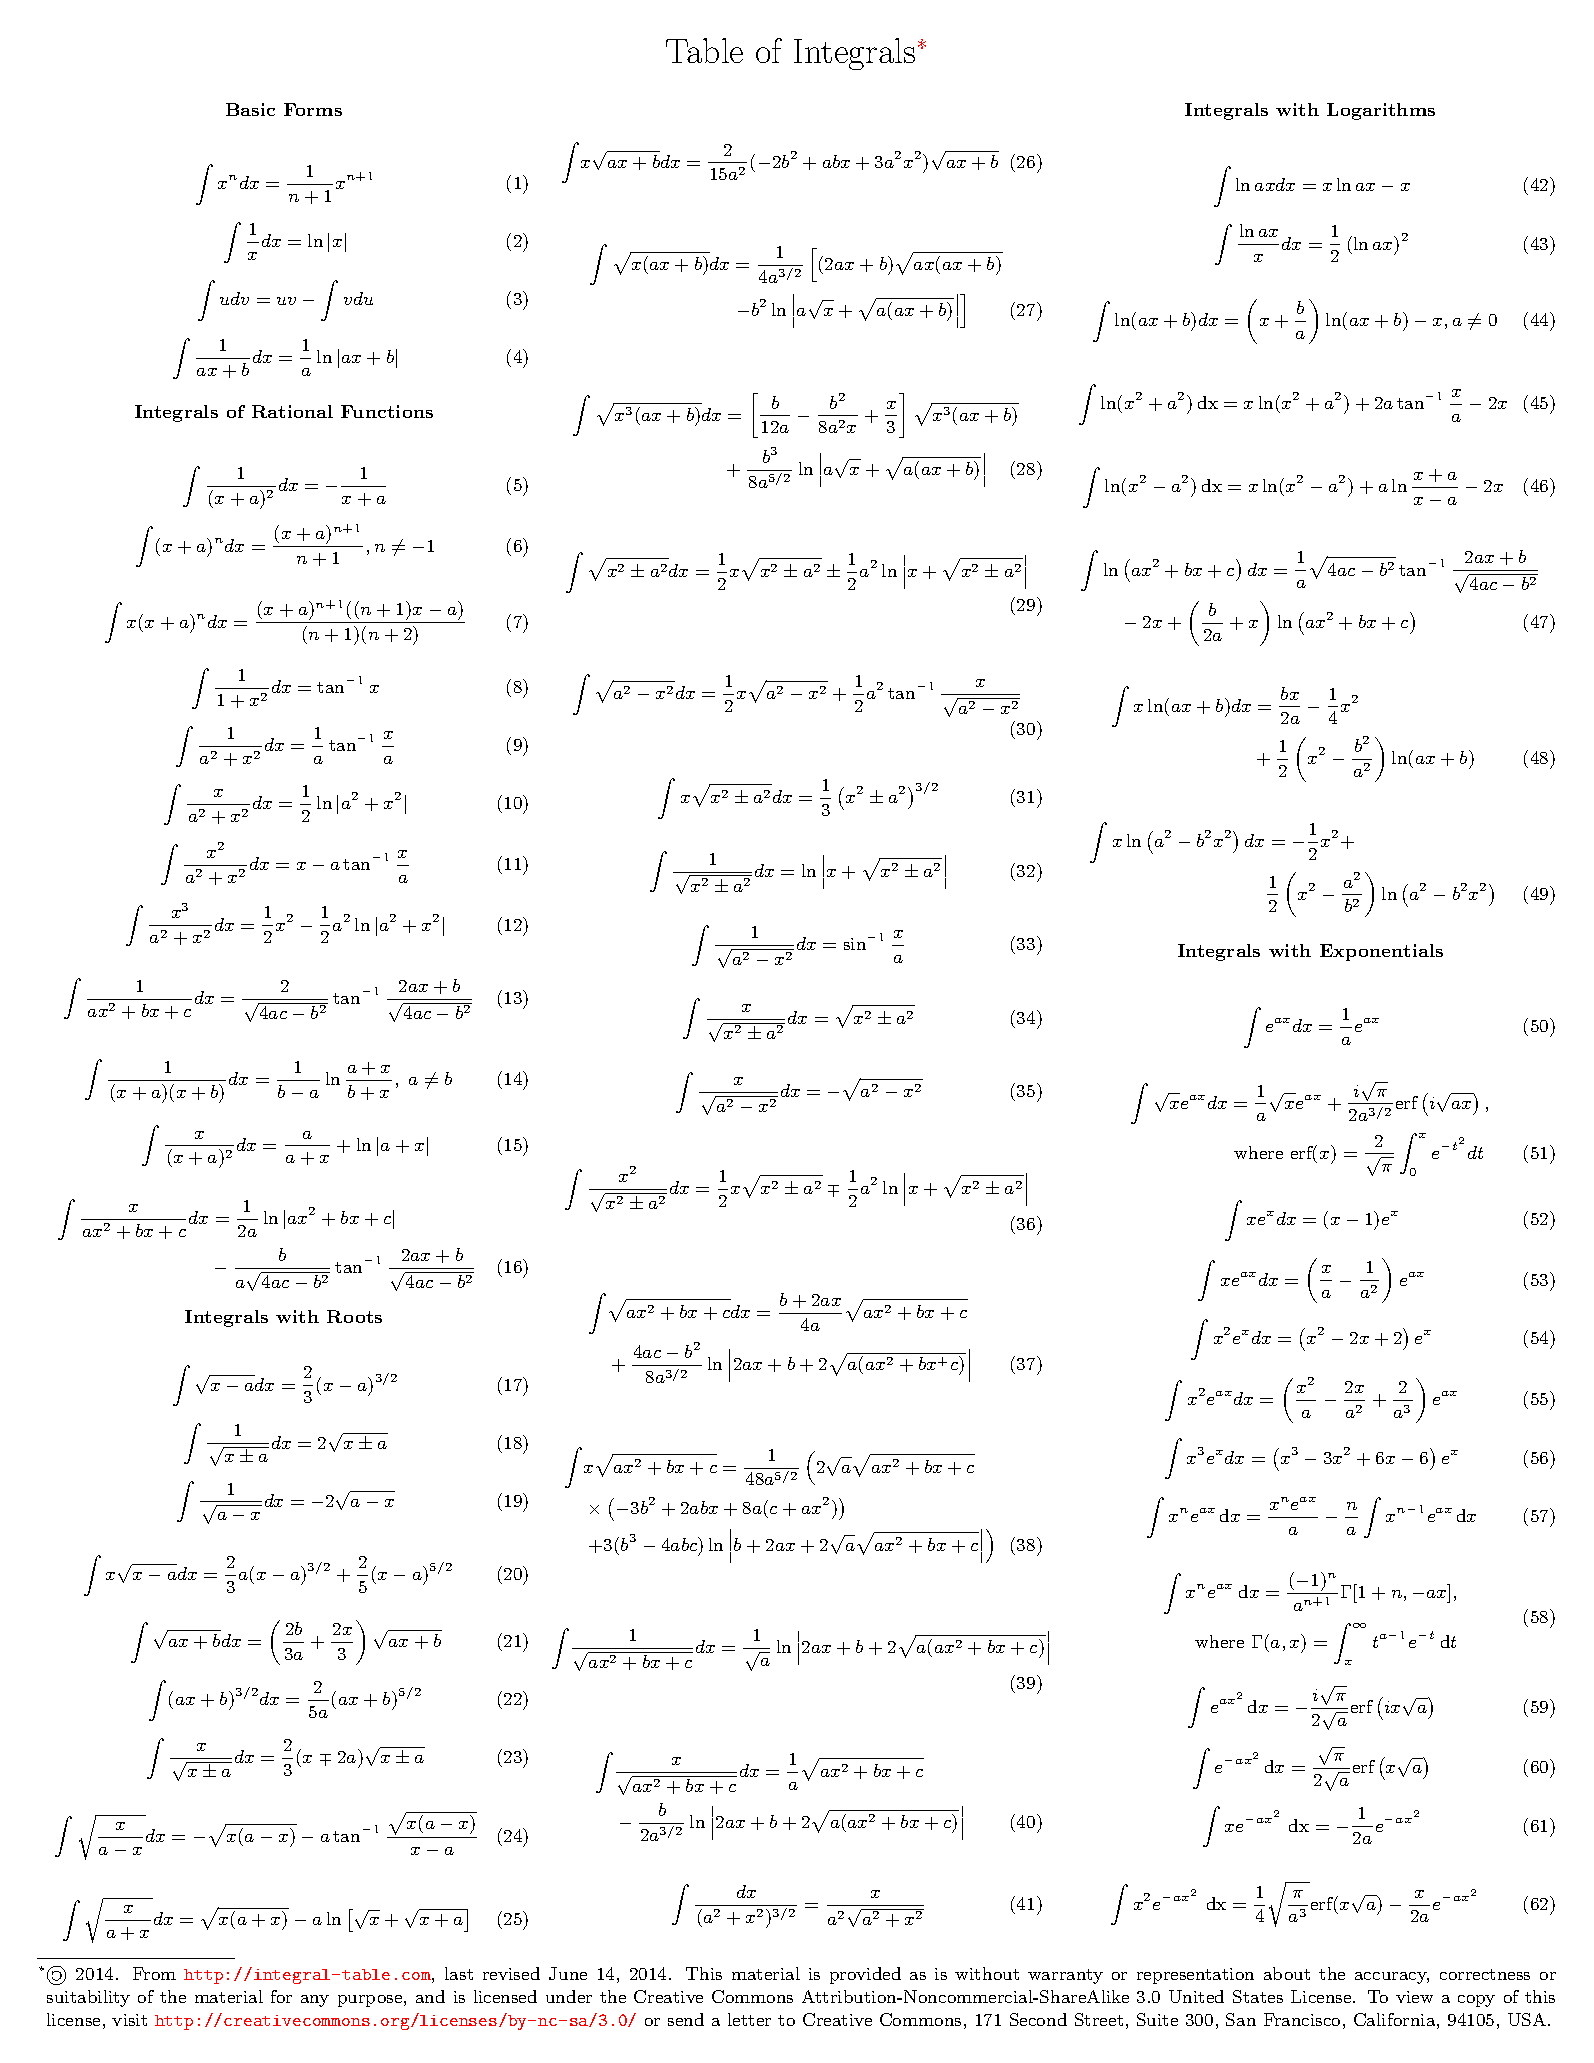
\includepdf[pages={1, 2}, pagecommand={\pagestyle{fancy}}]{integral-table}

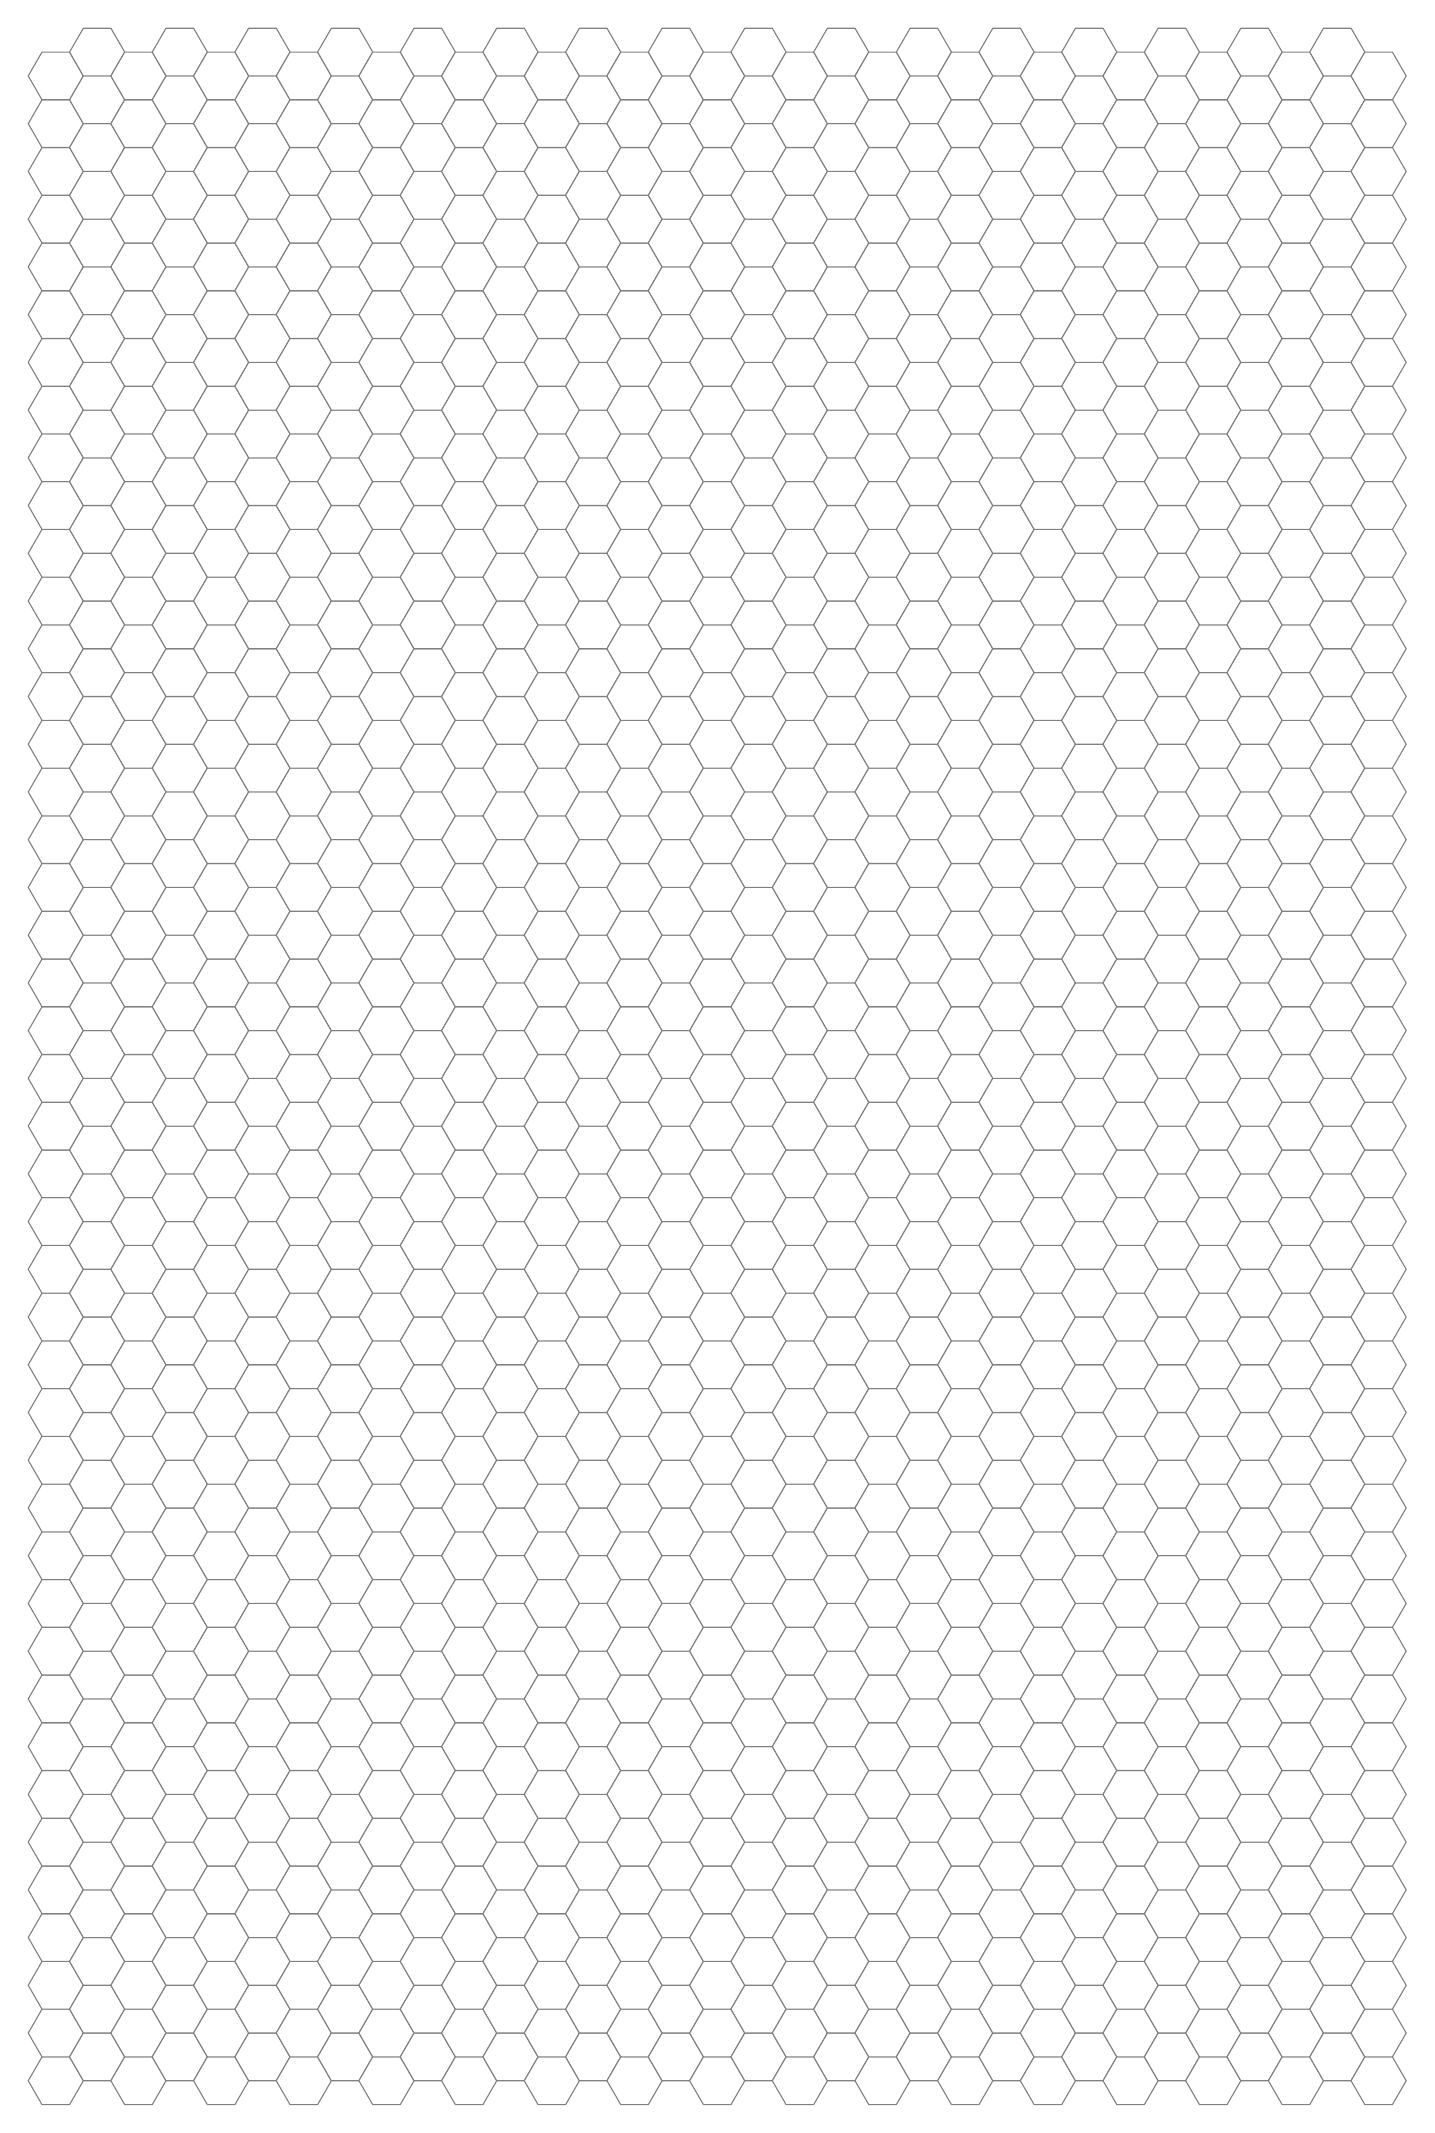
\begin{tikzpicture} [hexa/.style= {shape=regular polygon,
                                   regular polygon sides=6,
                                   minimum size=0.7cm, draw=gray,
                                   inner sep=0, anchor=south,
                                   fill=white}]

\foreach \j in {0,...,32}{% 
    \ifodd\j 
         \foreach \i in {0,...,42}{\node[hexa] (h\j;\i) at ({(\j/2+\j/4) * 0.7},{(\i+1/2)*sin(60) * 0.7}) {};}        
    \else
         \foreach \i in {0,...,42}{\node[hexa] (h\j;\i) at ({(\j/2+\j/4) * 0.7},{\i*sin(60) * 0.7}) {};}
    \fi}
\end{tikzpicture}

\end{document}
